\documentclass[12pt]{article}
\usepackage{amsmath, amssymb, amsthm, mathtools}
\usepackage{booktabs}
\usepackage{float}
\usepackage{enumerate}
\usepackage{tikz}
\usetikzlibrary{arrows.meta}
\usepackage[hidelinks]{hyperref}

\theoremstyle{plain}
\newtheorem{thm}{Theorem}
\newtheorem*{thm*}{Theorem}
\newtheorem{lem}[thm]{Lemma}
\newtheorem{cor}[thm]{Corollary}
\newtheorem{conj}{Conjecture}
\newtheorem{claim}[thm]{Claim}
\newtheorem*{claim*}{Claim}
\newtheorem{prob}{Problem}

\newtheorem{innernumberedthm}{Theorem}
\newenvironment{numberedthm}[1]
  {\renewcommand\theinnernumberedthm{#1}\innernumberedthm}
  {\endinnernumberedthm}
\providecommand{\innernumberedthmautorefname}{Theorem}
\providecommand{\numberedthmautorefname}{Theorem}


\theoremstyle{definition}
\newtheorem{defn}[thm]{Definition}
\newtheorem{prop}[thm]{Property}
\newtheorem{note}[thm]{Notes}
\newtheorem{ex}[thm]{Example}
\newtheorem{obj}{Objective}
\newtheorem{rem}[thm]{Remark}

\DeclareMathOperator{\lcm}{lcm}

\newenvironment{solution}{%
    \vspace{1em} % Add one line of vertical space
    \noindent\textit{Solution.}%
}{\par}

\title{Advanced Combinatorics}

\author{Vasu Menon}
\date{Budapest Semesters in Math \\ Autumn 2025}

\begin{document}

\maketitle

\tableofcontents % Generates a table of contents
\newpage

\section*{Syllabus}
\label{sec:syllabus}
\addcontentsline{toc}{section}{Syllabus}
\textbf{Instructor:} András Gyárfás\footnote{Alfréd Rényi Institute of Mathematics, Hungarian Academy of Sciences, Budapest, Hungary}

The course provides a comprehensive introduction to the theory of finite set systems (hypergraphs), exploring both classical foundations and modern developments. Emphasis is placed on fundamental proof techniques, particularly \textit{linear algebraic} and \textit{probabilistic} methods, that have shaped contemporary combinatorics.

\subsection*{Topics}

\begin{enumerate}[1.]
    
    \item \textbf{Basic Concepts:}  
    Incidence matrix, duality, intersection graphs, examples of hypergraphs (paths, cycles, linear spaces, Steiner systems, planar and intersecting linear spaces, finite projective planes).

    \item \textbf{Chromatic Number and Girth:}  
    Proper coloring and the greedy algorithm, extremal examples, classical constructions (Zykov, Mycielski, Tutte, Shift, Kneser graphs), hypergraph constructions via gluing, and the Neszetril-Rödl hypergraph.

    \item \textbf{Ramsey Theory:}  
    Ramsey numbers and their bounds (recursive and non-recursive), exact values, pigeonhole arguments, multicolor and non-diagonal variants, convex $n$-gons in planar point sets; Van der Waerden numbers; Tic-Tac-Toe and the Hales-Jewett theorem (including Shelah's proof); infinite combinatorics and applications.

    \item \textbf{Counting \& Probabilistic Methods:}  
    Proofs by counting (antichains, intersecting hypergraphs, 3-chromatic examples); Erdős's lower bounds for $R(n)$ and $W(k)$; probabilistic constructions, tournaments and transitive subtournaments, paradoxical tournaments (Klein-Szekeres bound); expectations and the probabilistic method in existence proofs; Local Lemma and its applications (Erdős-Lovász theorem, even cycles in regular digraphs); curiosities such as Spencer's injections and “triangle is 2-chromatic.”

    \item \textbf{Linear Algebra Methods:}  
    Dimension bounds (including Oddtown theorem, Fisher inequality), cubic lower bounds for $R(n)$, two-distance sets, cross-intersecting families; homogeneous linear equations in combinatorics (bipartite partitions of $K_n$, discrepancy of hypergraphs); eigenvalue techniques and extremal configurations (Hoffman-Singleton theorem, cages of girth five).

    \item \textbf{Special Topics:}  
    Systems of distinct representatives, chain decompositions, hypergraphs with $n$, $n+1$, and $n+2$ edges; critical 3-colorable hypergraphs; sunflower theorem and sum-free sets; factorizations of $K_n$ and Steiner triple systems.

    \item \textbf{Advanced Topics:}  
    Cyclic generators in Desarguesian planes, hypergraph factorization, two proofs of the Perfect Graph Theorem, constructive super-polynomial lower bounds for $R(n)$, geometric hypergraphs and Borsuk's conjecture, graphs with large chromatic number and girth, Paley graphs and Paley tournaments.

\end{enumerate}

\newpage

\section*{Set 1}
\label{sec:set1}
\addcontentsline{toc}{section}{Set 1}
\subsection*{Problem 1}
Decide if there exists a graph with the following degree sequence: 
\[
1,1,1,2,4,5,6,6,7
\]


\begin{solution}
There does not exist such a graph. The sum of the degrees of a graph's vertices must be even ($2|E|$), but here, the sum of the degrees is 33, which is odd.
\end{solution}

\subsection*{Problem 2}
Prove that any simple graph on at least 2 vertices contains two vertices having the same degree.

\begin{proof}
Suppose a simple graph $G = (V,E)$ has $n \geq 2$ vertices. Then for any $v \in V$, $d(v) \leq n-1$ and $d(v) \in \{ 0,\dots,n-1 \}$. Since we have $n$ vertices and $n-1$ degree ``options'', at least two vertices must fall in the same degree ``option''. Note that if $d(v)=0$ for some $v \in V$, then you cannot have another vertex $v' \in V$ with $d(v')=n-1$. Thus, there are at least two vertices having the same degree.
\end{proof}

\subsection*{Problem 3}
Verify that for any graph $G=(V,E)$, either $G$ or its compliment $\overline{G}$ is connected.

\begin{proof}
If $G$ is connected, then we are done. Otherwise, if $G$ is not connected, then there exist vertices $u,v \in V$ such that there is no path from $u$ to $v$. This implies that there are two subgraphs $A = (V_A, E_A)$ and $B = (V_B, E_B)$ of the graph $G = (V, E)$ such that $ V_A \cap V_B = \emptyset $ and $ V_A \cup V_B = V $ and for every $a \in V_A$ and $b \in V_B$, $ab \notin E$. Now, in the compliment $\overline{G} = (\overline{V}, \overline{E})$, for every $a \in V_A$ and $b \in V_B$, $ab \in \overline{E}$. Thus there exists paths between any vertex in $V_A$ and any vertex in $V_B$, and any vertices $u,v \in V_B$ has a path via a vertex in $V_A$ and any vertices $u,v \in V_A$ has a path via a vertex in $V_B$. So $\overline{G}$ is connected.
\end{proof}

\subsection*{Problem 4}
Prove that if $G=(V,E)$ is a simple graph on $2n$ vertices such that every vertex has degree at least $n$, then $G$ is connected.

\begin{proof}
We will proceed inductively. For the base case, assume $n=1$. A graph with 2 vertices with a connection between them is connected. Assume a simple graph on $2n$ vertices such that every vertex has degree at least $n > 1$ is connected. We will prove that a graph on $2(n+1)=2n+2$ vertices such that every vertex has at least degree $n+1$ is connected as well. We are taking the connected graph with $2n$ vertices and adding 2 additional vertices. We are also then taking each vertex and adding 1 to it's degree, effectively adding an edge that it previously did not have. Note that these 2 new vertices can either connect to itself, or connect to a vertex that exists within this connected section. Since these vertices each has degree at least $n+1$, each of them must connect back to the connected path of the graph. Thus, this newly constructed graph is connected as well.
\end{proof}

\subsection*{Problem 5}
Prove that any connected graph has a vertex whose deletion (together with the edges incident to it) results in a connected graph.

\begin{proof}
We know that the vertices of a connected graph $G$ can always be enumerated as $v_1, \dots, v_n$ so that 
$G_i := G[v_1, \dots, v_i]$ is connected for every $i$. Setting $i = n$, we have $G_n = G[v_1, \dots, v_n]$. Consider the vertex $v_n$. Deleting it results in the graph $G_{n-1} = G[v_1, \dots, v_{n-1}]$ which is still connected.
\end{proof}

\subsection*{Problem 6}
Prove that if $G=(V,E)$ is a graph with at least 5 vertices, then either $G$ or $\overline{G}$ contains a cycle.

\begin{proof}
If $G$ contains a cycle, then we are done. Otherwise, let $G$ be an n vertex graph without a cycle with $n>5$. Then $G$ is a forest with $1 \leq d \leq 5$ trees. 
We know then that the number of edges $|E_G| \leq n-1$. In $\overline{G}$, however, we have $|E_{\overline{G}}| = |E_{K_n}|-|E_G|= \frac{n(n-1)}{2} - |E_G| \geq \frac{n(n-1)}{2} + n - 1$ \footnote{We know $|E_{K_n}| = \frac{n(n-1)}{2}$ because given $n$ vertices, we first connect one of them to the other $n-1$ vertices, then another one to the remaining $n-2$ vertices and so on. In the end we have the sum $\sum_{1}^{n-1} = \frac{n(n-1)}{2} $.}.
Note then that for all $n>5$, $|E_{\overline{G}}| \geq \frac{n(n-1)}{2} + n - 1 > n - 1$. Since this compliment graph has greater than $n-1$ edges, it has more edges that it's spanning tree, and thus is no longer a tree and contains a cycle.
\end{proof}


\subsection*{Problem 7}
Determine the tree whose Prüfer code is $(4,4,7,4,1)$.

\begin{solution}
\begin{center}
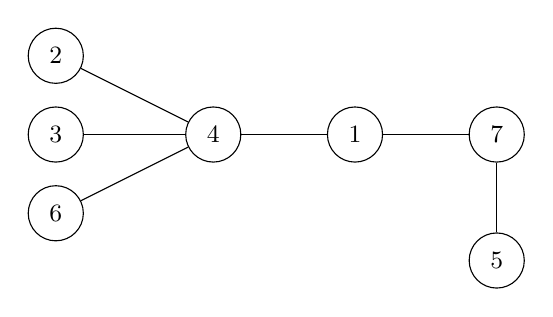
\begin{tikzpicture}[every node/.style={circle,draw,minimum size=7mm,font=\small}]
  \node (4) at (0,0) {4};
  \node (2) at (-2,1) {2};
  \node (3) at (-2,0) {3};
  \node (6) at (-2,-1) {6};
  \node (1) at (1.8,0) {1};
  \node (7) at (3.6,0) {7};
  \node (5) at (3.6,-1.6) {5};

  \draw (4)--(2);
  \draw (4)--(3);
  \draw (4)--(6);
  \draw (4)--(1);
  \draw (1)--(7);
  \draw (7)--(5);
\end{tikzpicture}
\end{center}
\end{solution}

\subsection*{Problem 8}
Characterize those trees whose Prüfer code consists of all different numbers.

\begin{solution}
If a tree with length $n$ has a Prüfer code has no repeating number, then the tree is just a straight path with length $n$. The code has length $n-2$. In the tree, there are 2 vertices with degree 1, and they don't appear in the code. The other $n-2$ vertices each appear once in the code, which means they have degree 2, and these are the inner vertices of the path. 
\end{solution}

\subsection*{Problem 9}
Let $T$ be a tree whose Prüfer code consists of the same number. What is the maximum length of a path in $T$?

\begin{solution}
If the Prüfer code of $T$ consists of the same number, then there is exactly one vertex (whose label is the only number in the Prüfer code) with many leaves. So the maximum length of a path in $T$ is 2, with this maximal path going from a leaf to the main node to another leaf.
\end{solution}

\subsection*{Problem 10}
Determine the number of trees on vertices $1, \ldots, n$ in which vertex 1 has degree exactly 2.

\begin{solution}
We can count the number of Prüfer codes (with length $n-2$) that represent this tree. Since vertex 1 has degree exactly 2, it appears exactly once in the code, and there are $n-2$ choices where it can go. We then have have $n-1$ other labels with $n-3$ positions where they can go. Thus, we have $(n-2)(n-1)^{n-3}$ such trees.
\end{solution}
\newpage

\section*{Set 2}
\label{sec:set2}
\addcontentsline{toc}{section}{Set 2}
Theorems used in the set (for reference):
\begin{numberedthm}{1.4}\label{thm:1.4}
Assume $\mathcal{H} = (\mathcal{V}, \mathcal{E})$ is an intersecting linear space not isomorphic to a trivial one or to a near pencil. Then (for some integer $k \geq 2$)
\[
    |\mathcal{E}| = |\mathcal{V}| = k^2 + k + 1, \quad \mathcal{H} \text{ is } (k+1)\text{-uniform and } (k+1)\text{-regular}
\]
\end{numberedthm}

\subsection*{Problem 6}
Work out the details of the proof of \autoref{thm:1.4}

\begin{proof}
Note that if one edge covers all of $V$, clearly then, $H$ is trivial. If there are two edges $e_1,e_2$ that cover all of $V$, due to the fact that $H$ is linear, they meet at a unique vertex $r$. Additionally, without loss of generality, we know one of the edges, say $e_2$, has size $2$. Then $e_1$ contains all but one vertex, and every other edge is an edge with 2 vertices joining $r$ to a vertex of $e_1$. Thus $H$ is a near-pencil.

\noindent Now, we will show that for the case where no 2 edge cover all of $V$, a linear intersecting space $G$ implies that $|V|=|E|=k^2+k+1$ where $G$ is $(k+1)$-uniform and $(k+1)$-regular. Consider $e_1,e_2 \in E$ and suppose $v \in V$ is a vertex such that $v \notin e_1 \cup e_2$. By the definition of linear spaces, every vertex in $e_1$ must be conected to $v$ by a unique edge, and such an edge must not intersect with both $e_1$ and $e_2$. Thus, there exists a bijection between every vertex $v \in e_1$ to another edge that must contain $v$ and one unique vertex in $e_2$. Note that we cannot have the case where such an edge contains more than one unique vertex from $e_1$ and $e_2$ since it would thus violate the conditions of a linear space by creating 2 edges that contain both vertices in $e_1$ or $e_2$. Therefore, $|e_1| = |e_2|$, and thus all edges have the same size.
Next, we will show that $d(v)=|e|$ for any $e \in E$ and $v \in V$. Suppose $G$ is an intersecting linear space. Choose $e \in E$ and $v \in V$ such taht $v \notin e$. Since $G$ is linear, there must be a unique edge containing $v$ and every other vertex in $e$, and thus, $d(v) \geq |e|$. Assume for the sake of contradiction that $d(v) > |e|$. This implies that there exists $v_1 \in V$ such that $v_1 \notin e$ and $e_1$ such that $v, v_1 \in e_1$. Note that the fact that the edge containing $v, v_1$ cannot intersect with the edge $e$ without violating the definition of a linear space, and thus, no such extra edge exists and $d(v)=|e|$.
Finally, we will show that $G$ being $(k+1)$-uniform and $(k+1)$-regular implies $|V|=|E|=k^2+k+1$. For every vertex $v$, note that there are $k+1$ edges containing it. Each $k+1$ edges has $k$ vertices contained in it excluding $v$. Thus, there are $k(k+1)$ other vertices. With $v$, there are $k(k+1)+1=k^2+k+1$ vertices, and thus, $|V|=|E|=k^2+k+1$.
\end{proof}

\subsection*{Problem 7}
The Fano plane has cyclic representation: shift the set \{1,2,4\} (by adding 1 to its elements) six times, using arithmetic (mod 7). Find similar representations for the finite plane of order 3 and order 4.

\begin{solution}
For a finite plane of order $k$, we need to find a subset $S \subset Z_{k^2+k+1}$ with size $k+1$ such that no two ordered pairs in $S$ have the same difference using arithmetic (mod $k^2+k+1$). Instead of guess and check, we will use the following program to find such a subset.
\begin{verbatim}
import itertools

k = 3
num = k**2 + k + 1
Z = list(range(num))

for subset in itertools.combinations(Z, k+1):
    diffset = set()
    for i in subset:
        for j in subset:
            if i != j:
                diffset.add((i - j) % num)

    if len(diffset) == num-1:
        print(subset)
        break


\end{verbatim}
We find that for order 3, the representation is the set $\{0, 1, 3, 9\}$
and for order 4, the representation is the set $\{0, 1, 4, 14, 16\}$
\end{solution}

\subsection*{Problem 8}
Suppose that $\mathcal{H} = (V,\mathcal{E})$ has no singleton edges and $|e \cap f| \ne 1$ for all $e,f \in \mathcal{E}$. Prove that in every ordering of $V$ the greedy algorithm colors $V$ with at most two colors. The proof cannot be longer than three sentences!

\begin{proof}
Suppose for the sake of contradiction that the algorithm uses color with label 3 at a vertex $v$, and thus, there must be edges $e,f$ that contain $v$ with all vertices in $e$ colored with label 1 and all vertices in $f$ colored with label 2. Since there are no singleton edges, $e$ and $f$ have other vertices other than $v$, and they cannot be disjoint since then $e \cap f = \{v\}$, so they meet at some other vertex $u$. But since $u$ is either colored with a 1 or a 2, one of $e$ or $f$ cannot be monochromatic, which is a contradiction.
\end{proof}

\subsection*{Problem 9}
Prove that Steiner triple systems have no proper 2-colorings.

\begin{proof}
Assume for the sake of contradiction that a Steiner triple system of order $k$ has a proper 2-coloring. We will suppose that the two colors are the integer labels 1 and 2.
Without loss of generality, suppose we choose a vertex $a$ with color 1, and let the set of $B$ be the set of vertices colored 2.
Consider all triples containing $a$. 
Note that in a proper 2-coloring, each triple containing $a$ would include exactly one vertex that is colored 1. Additionally, every pair of vertices appears exactly in one triple. Thus, for each pair $\{a, b\}$ with $b \in B$, there is a triple containing both $a$ and $b$, and so for each $b \in B$, the triple containing $a$ and $b$ is determined by the pair $\{a, b\}$.
Since each triple containing $a$ contains exactly 2 pairs, and since there are $v-1$ total pairs, $a$ is contained in $\frac{v-1}{2}$ triples. Since $a$ is colored 1, each of these triples must contain exactly one vertex colored 2. Thus, $|B| = \frac{v-1}{2}$. Since same argument above applies to any vertex colored 2, supposing that $A$ is the set of vertices colored 1, we have that $|A| = \frac{v-1}{2}$. Then the total number of vertices is $|A| + |B| = \frac{v-1}{2} + \frac{v-1}{2} = v - 1 \neq v$, which is a contradiction. Therefore, no proper 2-coloring exists for a Steiner triple system.
\end{proof}


\subsection*{Problem 10}
Prove that finite planes of order at least 3 have proper 2-colorings.

\begin{proof}
Suppose we have a finite plane of order $k \geq 3$. Within this plane, we have a set of vertices $V$ and edges $E$ each edge contains $e+1 \geq 4$ vertices. We will then color the vertices with labels that are either a 1 or a 2. Suppose we choose an edge $e \in E$ and color one vertex with a 1 and the rest with a 2. Then, if we take any other vertex on $e$ and look at the other edge $f$ that contains it, we can observe that there are $k+1$ vertices on $f$. Thus, there are at least $3$ other uncolored vertices. Choose a vertex on $f$ and give it the color 1, and the rest the color 2. Repeating this process throughout entire finite planes will provide it a proper 2-coloring since every edge intersects our initial edge $e$ at exactly one vertex. Since $k \geq 3$, there are at least 3 additional vertices to color such that the edge contains both colors. Since every new edge contains at least one previously colored vertex, we can always color remaining points to avoid monochromatic edges. Therefore every edge will contain at least one vertex colored with a 1 and one vertex colored with a 2, so we have a proper 2-coloring.
\end{proof}
\newpage

\section*{Set 3}
\label{sec:set3}
\addcontentsline{toc}{section}{Set 3}
\subsection*{Problem 1}
Prove that Pósa's theorem implies Ore's theorem

\begin{proof}
For a graph $G=(V,E)$, assume Ore's theorem's condition, that is, assume $d(u)+d(v) \geq n$ for every $u,v \in V$ with $uv \notin E$. Since $uv \notin E$, then $d(u) \leq n-2$, since $u$ cannot be connected to itself and the vertex $v$. Similarly, $d(v) \leq n-2$. Thus, $d(u)+d(v) \leq 2n-4$, and since $d(u) \geq 1$ and $d(v) \geq 1$, we have that $d(u)+d(v) \geq 2$. This implies that $2 \leq d(u)+d(v) \leq 2n-4 \implies 2 \leq 2n-4 \implies n \geq 3$. Now, suppose $1 \leq d_1 \leq d_2 \leq \dots \leq d_n < n$ is the degree sequence. Then, for all $i < j \leq \frac{n}{2}$, $i+j < n$, and since we know that by Ore's condition, $d_i + d_j \geq n$, we have that $i < j \leq i+j < n \leq d_i + d_j$, and thus, $i < j < d_i + d_j$. This implies that for all $d_i \geq i+1$, which is exactly Pósa's condition, and thus, there exists a Hamilton cycle. Therefore, Pósa's theorem implies Ore's theorem.
\end{proof}

\subsection*{Problem 2}
Let $G$ be a graph on $2x+1$ vertices with all degrees at least $x$. Prove that $G$ contains a Hamilton path.

\begin{proof}
Suppose $G$ is a graph with $n=2x+1$ vertices and all vertices have degree at least $x$. Now, add a vertex $v_0$ and connect it to all $2x+1$ vertices, and thus, $d(v_0)=2x+1$. Consequently, we have $n=2x+2$ vertices such that for every vertex $v \in V$, $d(v) \geq x+1 = \frac{2x+2}{2} = \frac{n}{2}$. Thus, by Dirac's theorem, we have a Hamilton cycle. Removing the vertex $v_0$ from the graph would then leave it without a Hamilton cycle, but a Hamilton path would exist.
\end{proof}

\subsection*{Problem 3}
Let $G$ be a regular simple graph on $2025$ vertices that contains a Hamilton cycle. Prove that $G$ also contains a Eulerian circuit. (Reminder: We say that a graph is regular if all of its vertices have equal degree.)

\begin{proof}
Suppose $G$ is a regular simple graph with $2025$ vertices that contains a Hamilton cycle. To prove that $G$ also contains an Eulerian circuit, we need to show that $G$ is connected and that every vertex in $G$ has an even degree. Since $G$ contains a Hamilton cycle, then we know it must be connected. Furthermore, since the graph is regular, suppose each vertex has degree $d$. Then, for 2025 vertices, the sum of the degrees, $\sum{d(v)}=2025d$. By the Handshake Lemma, we know that this sum must be even, and thus, $d$ must be even. Therefore, $G$ also contains a Eulerian circuit.
\end{proof}

\subsection*{Problem 4}
An oriented complete graph is called a tournament. Show that every tournament contains a directed Hamilton path.

\begin{proof}
We will proceed by induction. For the base case, consider a tournament with 1 vertex. Trivially, there exists a directed Hamilton path. Now for the inductive step, suppose the tournament with $n$ vertices contains a directed Hamilton path enumerated as $v_1, v_2, \dots, v_n$. Consider adding a vertex $u$ and ensuring that all other vertices have a directed edge connecting it. If we have all other vertices outwardly pointing to $u$, then there exists the Hamilton path $v_1, v_2, \dots, v_n, u$. If $u$ has outwardly directed edges to all other vertices, then there exists the Hamilton path $u, v_1, v_2, \dots, v_n$. Consider the first vertex in the sequence $v_1, v_2, \dots, v_n$ that $u$ has an outward edge pointing to. Call this vertex $v_i$. Note that then, $v_{i-1}$ points to $u$, and thus, there exists the Hamilton path $v_1, v_2, \dots, v_{i-1}, u, v_i, \dots, v_n$. Therefore, every tournament contains a directed Hamilton path.
\end{proof}

\subsection*{Problem 5}
Suppose that a graph $G$ can be partitioned into $k$ edge-disjoint spanning trees. Let $s$ be a specified node of $G$. Prove that $G$ can be partitioned into $k$ edge-disjoint spanning trees $T_1,\dots, T_k$ in such a way that the trees are equitable at $s$ in the sense that $|d_{T_i}(s) - d_{T_j}(s)| \leq 1$ for every $i, j \in [k]$.

\begin{proof}
TODO
\end{proof}
\newpage

\section*{Set 4}
\label{sec:set4}
\addcontentsline{toc}{section}{Set 4}
\subsection*{Problem 1}
Let $D = (V, A)$ be a directed graph and let $c : A \to \mathbb{R}$ be a conservative weight function. Is it true that there always exists a nonnegative feasible potential?

\begin{proof}
Yes. Let $n = |V|$ and let $s \in V$ be some vertex. Suppose $\pi(v) \coloneq \min(\text{cost of a walk from s to v with at most } n-1 \text{ edges})$. Consider an edge $uv \in A$ and take the minimum walk from $s$ to $u$ with at most $n-1$ edges (which has cost $\pi(u)$) and add the edge $uv$ to the walk. Now we have a walk from $s$ to $v$ with a cost $\pi(u) + c(uv))$ and therfore, $\pi(v) \leq \pi(u) + c(uv)$. Rearranging yields $\pi(v)-\pi(u) \leq c(uv)$ and thus, $\pi$ is a feasible potential. Now, let $\pi'(v) \coloneq \pi(v) - m$ where $m$ is the minimum faesible potential among all vertices. Here, we have that $\pi'(v) \geq 0$ for all $v \in V$ and is thus a nonnegative feasible potential, and therefore, there always exists a nonnegative feasible potential.
\end{proof}

\subsection*{Problem 2}
Let $D = (V, A)$ be a directed graph and let $c : A \to \mathbb{R}$ be a conservative weight function. Is it true that any subpath of a cheapest $s$-$t$ path is itself a cheapest path between its endpoints?

\begin{proof}
Yes. Let $\mu(s\text{-}t)$ be the minimum cost of an $s$-$t$ path. Let $u \in V$ be a vertex contained inside of this path. Here, $s$-$u$ is an arbitrary subpath of the $s$-$t$ path. Then, since $C(s\text{-}t)=\mu(s\text{-}t)$, we have that $\mu(s\text{-}t) = C(s\text{-}u) + C(u\text{-}t)$ where $C$ denotes the cost of a path. Note that since $c$ is conservative, there are no negative cycles, and $C$ is therefore well-defined. If $C(s\text{-}u)$ was not the minimum cost of an $s$-$u$, then $\mu(s\text{-}t)$ would no longer be minimal, thus, $C(s\text{-}u)=\mu(s\text{-}u)$. Therefore, $\mu(s\text{-}u)$ is the cost of the cheapest $s$-$u$ path, which is some subpath of the $s$-$t$ path.
\end{proof}

\subsection*{Problem 3}
Let $D = (V, A)$ be a directed graph and let $c : A \to \mathbb{Z}$ be a conservative weight function. Suppose $\pi_1$ and $\pi_2$ are both feasible potentials with respect to $c$.
\begin{enumerate}[\indent(a)]
    \item  Prove that $\lfloor (\pi_1 + \pi_2)/2 
    \rfloor$ and $\lceil (\pi_1 + \pi_2)/2 \rceil$ are also feasible potentials.
    \item Prove that $\max(\pi_1, \pi_2)$ and $\min(\pi_1, \pi_2)$ are feasible potentials.
\end{enumerate}

\begin{proof}
Assume $\pi_1(v) - \pi_1(u) \leq c(uv)$ and $\pi_2(v) - \pi_2(u) \leq c(uv)$ for all edges $uv \in A$
\begin{enumerate}[\indent(a)]
    \item Define $\pi_{avg} \coloneq \frac{\pi_1+\pi_2}{2}$. Then, summing up the two inequalities in our assumption and dividing by 2 yields $\frac{\pi_1(v)+\pi_2(v)}{2} - \frac{\pi_1(u)+\pi_2(u)}{2} \leq c(uv)\implies \pi_{avg}(v) - \pi_{avg}(u) \leq c(uv)$, and thus, $\pi_{avg}$ is feasible. Now, since the costs are integers, we have that $\lfloor \pi_{avg}(v) \rfloor - \lfloor \pi_{avg}(u) \rfloor \leq \pi_{avg}(v) - \pi_{avg}(u) \leq c(uv)$ and that $\lceil \pi_{avg}(v) \rceil - \lceil \pi_{avg}(u) \rceil \leq \pi_{avg}(v) - \pi_{avg}(u) \leq c(uv)$. Thus, $\lfloor (\pi_1 + \pi_2)/2 
    \rfloor$ and $\lceil (\pi_1 + \pi_2)/2 \rceil$ are feasible potentials.
    \item Define $\pi_{max}(v) \coloneq \max(\pi_1(v), \pi_2(v))$. Note that for any edge $uv \in A$, $\pi_{max} \leq \max(\pi_1(u) + c(uv), \pi_2(u) + c(u,v))$. Since $c(uv)$ is a constant, we have that $\max(\pi_1(u) + c(uv), \pi_2(u) + c(u,v)) = \pi_{max}(u)+c(uv)$. This implies that $\pi_{max}(v) \leq \pi_{max}(u) + c(u,v) \implies \pi_{max}(v) - \pi_{max}(u) \leq c(u,v)$, and thus, $\pi_{max}$ is a feasible potential. We will proceed similarly for $\pi_{min} \coloneq \min(\pi_1(v), \pi_2(v))$. Observe that $\pi_{min}(v) \leq \min(\pi_1(u) + c(uv), \pi_2(u)+c(uv)) \implies \min(\pi_1(u)+c(uv),\pi_2(u)+c(uv)) = \pi_{min}(u) + c(uv)$. So, $\pi_{min}(v) \leq \pi_{min}(u) + c(uv)$ and therefore, $\pi_{min}(v)-\pi_{min}(u) \leq c(uv)$. Thus, $\pi_{min}$ is a feasible potential as well.
\end{enumerate}
\end{proof}

\subsection*{Problem 4}
Let $D = (V, A)$ be a directed graph and let $c : A \to \mathbb{Z}$ be a conservative weight function. Furthermore, let $P$ be a cheapest $s$-$t$ path. Reverse the edges of $P$ and negate the costs of these edges. Show that the resulting cost function is also conservative in the graph thus obtained.

\begin{proof}
TODO
\end{proof}

\subsection*{Problem 5}
Develop an algorithm to decide whether a directed graph with a conservative weight function contains a zero-weight cycle.

\begin{proof}
TODO
\end{proof}

\subsection*{Problem 6}
Given a directed graph with a conservative weight function on the edges and a lower and upper bound specified for each vertex, how can one decide whether there exists a feasible potential within the given bounds?

\begin{proof}
We need to find way to detect if there exists a $\pi$ such that $\pi(v) - \pi(u) \leq c(u,v)$ and $l(v) \leq \pi(v) \leq u(v)$ for all $v \in V$. To do so, apply the following process:

\noindent Consider a vertex $v_0$ with $\pi(v_0)=0$. Then, $\pi(v) \leq u(v) \implies \pi(v) - \pi(v_0) \leq u(v)$. Moreover, $\pi(v) \geq l(v) \implies \pi(v_0) - \pi(v) \leq -l(v)$. Consider these differences as directed edges on a graph, since they are of the same form as the feasible potential constraint $\pi(v) - \pi(u) \leq c(u,v)$. 
Represent the inequality $\pi(v) - \pi(v_0) \leq u(v)$ as an edge from $v_0$ to $v$ with cost u(v), and represent the inequality $\pi(v_0) - \pi(v) \leq -l(v)$ as an edge from $v$ to $v_0$ with cost $-l(v)$. Note that in this graph, if there exists a negative cycle, then $\pi$ is unfeasable and thus, there does not exist a feasible potential within the given bounds. Therefore, we must now detect the existence of negative cycles precisely by using the Bellman-Ford algorithm. If Bellman-Ford detects a negative cycle, no feasible potential exists, otherwise, there is a feasible potential within the given bounds.
\end{proof}

\subsection*{Problem 7}
Let $P$ be a path, and let $\mathcal{F}$ be a family of its subpaths. Develop an algorithm that select a collection of edge-disjoint subpaths from $\mathcal{F}$ so that the total length of the selected subpaths is maximized.

\begin{solution}
The algorithm will run as follows. First, take $\mathcal{F}$ and sort it so that each subpath is ordered based on the position of its ending vertex in $P$ where the smallest ending vertex is first. Then, initialize an empty list and iterate through every subpath $s$. Add $s$ to a list if $s$ does not share any edges with subpaths already in the list, otherwise, skip it. The collection of subpaths in the list will be the selection of edge-disjoint subpaths from $\mathcal{F}$ such that the total length of the selected subpaths is maximized.
\end{solution}

\subsection*{Problem 8}
Let $D = (V, A)$ be a directed graph and let $c : A \to \mathbb{Z}$ be a conservative weight function. Recall that $\pi_{c}^{n}(v)$ denotes the minimum cost of a walk of length at most $n$ ending at $v$. Prove that among all nonpositive feasible potentials, $\pi_{c}^{n}(v)$ is the largest; that is, for any feasible potential $\pi$, we have $\pi(v) \leq \pi_{c}^{n}(v)$ for all $v \in V$.

\begin{proof}
Let $\pi$ be a nonpositive feasible potential. Let $W=(v_0, v_1,\dots,v_k)$ with $v_k = v$ and $k \leq n$ denote a walk of length at most $n$ ending at $v$. We know that $\pi(v_i)-\pi(v_{i+1}) \leq c(v_i, v_{i+1})$ for all $i$. Then, $\pi(v)-\pi(v_0) \leq \sum_{i=0}^{k-1} c(v_i, v_{i+1}) = C(W)$. Since $\pi$ is nonpositive, we have that $\pi(v_0) \leq 0$ and thus $\pi(v) \leq C(W)$. Since this holds for all walks of length at most $n$ ending at $v$, it also holds for the minimum cost walk, and thus, $\pi(v) \leq \pi_{c}^{n}(v)$ for all $v \in V$.
\end{proof}
\newpage

\section*{Set 5}
\label{sec:set5}
\addcontentsline{toc}{section}{Set 5}
\subsection*{Problem 21}
Assume that $n \geq 3r!$. Prove that every $r$-coloring of the numbers in $[n]$ there is $x,y,z \in [n]$ such that they have the same color and $x+y=z$ ($x=y$ is permitted).

\begin{proof}
Consider the complete graph $K_{n+1}$ on vertices $V = \{0, 1, 2, \dots, n\}$. 
For each pair of vertices $\{i, j\}$ with $i < j$, color the edge $\{i, j\}$ by the color assigned to the integer $j - i$ in the given coloring of $[n]$. This defines an $r$-coloring of the edges of $K_{n+1}$. Next, note that from HW \#14, we know that $R(3,\dots,3 \text{ ($r$ times)}) \le 3r! \le n+1$. By the definition of the Ramsey number, every $r$-coloring of the edges of $K_{n+1}$ must contain a monochromatic triangle. Let the vertices of this monochromatic triangle be $a < b < c$. 
Since the triangle is monochromatic, all three edges $\{a, b\}$, $\{b, c\}$, and $\{a, c\}$ have the same color. From the way we colored the edges, this means that the three differences $b - a, c - b, c - a$ are all assigned the same color in $[n]$. But these satisfy the equation $(b - a) + (c - b) = c - a$. Thus, if we set $x = b - a$, $y = c - b$, and $z = c - a$, then $x, y, z \in [n]$ are of the same color and satisfy $x + y = z$.
\end{proof}

\subsection*{Problem 22}
Prove that the vertices of any transitive tournament $T_n$ can be labeled with $1,2,\dots,n$ so that each edge is oriented from a smaller label to a larger label.

\begin{proof}
We will proceed by induction. For the base case $n=1$, the statement is trivial. For the inductive hypothesis, assume that the statement holds for some $n-1 \geq 1$. Now let $T_n$ be a transitive tournament on $n$ vertices. Note that a transitive tournament does not contain cycles, and thus has a ``start'' vertex (a source) and an ``end'' vertex (a sink)\footnote{For a transitive tournament $T$, pick any vertex $x$. If $x$ is not a source, then there exists a vertex $u_1 \to x$. If $u_1$ is not a source, then there exists a $u_2 \to u_1$ and so on. Because the tournament does not contain a cycle, this sequence must terminate, and thus, we must reach a vertex with no incoming edges, which is the source. Similarly, there exists a vertex with no outgoing edges, which is the sink.}. Now, let $v_{\text{min}}$ be the source and let $v_{\text{max}}$ be the sink. Consider removing the sink to yield $T_n - v_{\text{max}}$, which is still a transitive tournament on $n-1$ vertices. By our inductive hypothesis, we can label the vertices $T_n - v_{\text{max}}$ with labels $1, \dots, n-1$ such that all edges go from smaller to larger labels. Now if we put $v_{\text{max}}$ back, all edges can go into it, and thus we can assign  $v_{\text{max}}$ the largest label $n$, preserving the property that every edge goes from smaller to larger label. By induction, the claim holds for all $n \geq 1$. Thus, the vertices of any transitive tournament $T_n$ can be labeled with $1,2,\dots,n$ so that each edge is oriented from a smaller label to a larger label. 
\end{proof}

\subsection*{Problem 23}
Prove that every tournament has a king: a vertex where any other vertex can be reached by a directed path with at most two edges.

\begin{proof}
Let $v$ be a vertex of maximum outdegree (the number of vertices with an incoming edge from $v$) in the tournament. Let $d$ be this outdegree. Define the set $\Gamma(v) = \{u : v \to u\}$ as the set of all vertices that have an incoming edge from $v$. Clearly, $|\Gamma(v)| = d$. Suppose, for the sake of contradiction, that there is a vertex $w$ that is not reachable from $v$ by any path of length $\leq 2$. That means the edge $v \to w$ does not exist and thus $w \to v$ exists, and no vertex $u \in \Gamma(v)$ has the edge $u \to w$ and thus for every $u \in \Gamma(v)$, we have $w \to u$. Therefore, $w$ has directed edges to $v$ and to every vertex in $\Gamma(v)$, and so the outdegree of $w$ is at least $d+1$. This contradicts the fact that $v$ is a vertex of maximum outdegree $d$. Thus, no such $w$ exists and every vertex is at distance at most $2$ from $v$, implying that $v$ is a king.
\end{proof}

\subsection*{Problem 24}
A tournament is called \textit{strong} if there is a directed path from any vertex to any other. Prove that any strong tournament has a directed Hamiltonian cycle.

\begin{proof}
First, we will show that every tournament on $n$ vertices has a Hamiltonian path. We proceed by induction on the number of vertices $n$. For the base case $n = 1$ the statement is trivial. For the inductive step, suppose that every tournament on $n-1$ vertices has a Hamiltonian path. Let $T$ be a tournament on $n$ vertices, and remove an arbitrary vertex $v$. By the induction hypothesis, $T - v$ has a Hamiltonian path $P = u_1 \to u_2 \to \cdots \to u_{n-1}$. Now insert $v$ into this path. If $v \to u_1$, then $v \to u_1 \to u_2 \to \cdots \to u_{n-1}$ is a Hamiltonian path of $T$. Otherwise, there exists an index $i$ with $u_i \to v$ and $v \to u_{i+1}$. Then $u_1 \to \cdots \to u_i \to v \to u_{i+1} \to \cdots \to u_{n-1}$ is a Hamiltonian path of $T$. Such an $i$ must exist since each pair of vertices is connected in exactly one direction. Thus, every tournament on $n$ vertices has a Hamiltonian path.
\\
\noindent Now, let $T$ be a strong tournament, and let $P = v_1 \to v_2 \to \cdots \to v_n$ be a Hamiltonian path (which we showed above). If $v_n \to v_1$ is an edge, then $v_1 \to v_2 \to \cdots \to v_n \to v_1$ is already a Hamiltonian cycle. Otherwise, assume $v_1 \to v_n$. Since $T$ is strong, there exists a directed path from $v_n$ back to $v_1$: $v_n = w_0 \to w_1 \to \cdots \to w_k = v_1$. Let $w_j$ be the first vertex on this path that also belongs to the Hamiltonian path $P$. Then $w_j = v_i$ for some $1 \le i \le n-1$. The edge entering $v_i$ on the path above is $w_{j-1} \to v_i$. Now, one of the two edges $v_{i-1} \to w_{j-1}$ or $w_{j-1} \to v_{i-1}$ must exist in $T$. In either case, we can connect the paths together to obtain a directed cycle containing all vertices: $v_1 \to \cdots \to v_{i-1} \to w_{j-1} \to \cdots \to v_n \to v_1$. Thus, $T$ contains a directed Hamiltonian cycle.
\end{proof}


\subsection*{Problem 25}
Assume (a real life situation) that ``knowing each other'' is not necessarily symmetric. Prove that at a party of nine persons one can always find either three strangers (no one knows any other) or three persons A,B,C such that A knows B and C and B knows C (a transitive triple). Show that the statement is not true for eight persons.

\begin{proof}
First, consider $R(3,4) \leq 9$. Suppose we utilize the colors white and black and an unoriented graph. Here, we know that any coloring of $K_9$, there exists a monochromatic (white) triangle ($K_3$) or a monochromatic (black) ``complete square'' ($K_4$). Consider each vertex as a person and white edges as ``not knowing each other'' and black edges as ``knowing each other''. Clearly, at a party of nine persons, there are three strangers who do not know each other (due to the existence of the white triangle). Additionally, there are four strangers that are part of a ``complete square'' ($K_4$). Consider the four vertices of this clique $\{a,b,c,d\}$. To prevent transitivity, we will construct cycles. Orient $a \to b \to c \to a$. Next, orient $b \to d \to a$. The edge between $c$ and $d$ are now unconnected, but any orientation of $c$ and $d$ (both $c \to d$ and $d \to c$) will result in $\{b,c,d\}$ being a transitive triple. Thus, orienting this 4 vertex clique $K_4$ will always result in a transitive triple.
\\
\noindent Now, to show that the statement is not true for eight persons, consider the following graph with $8$ vertices:

\begin{center}
    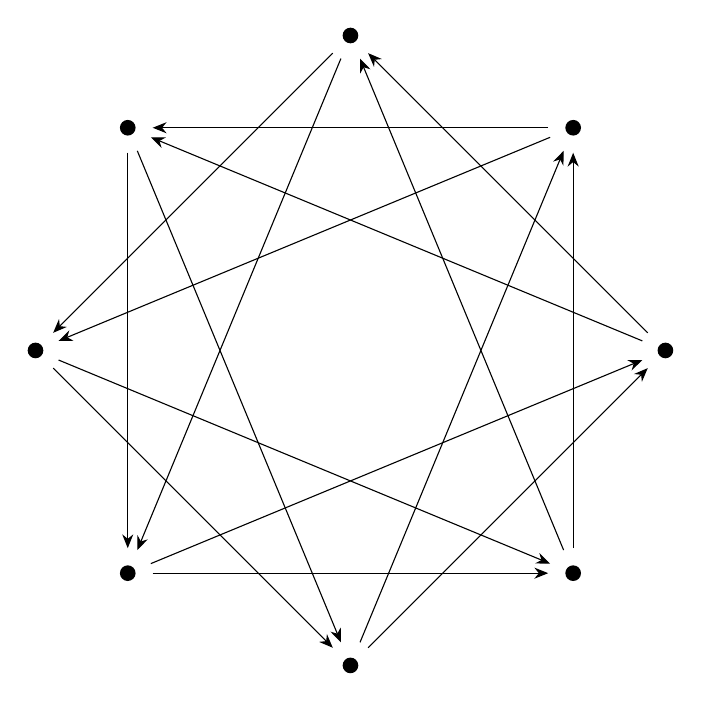
\begin{tikzpicture}[scale=2,
    every node/.style={circle,fill=black,inner sep=2pt},
    ->,
    >=Stealth,
    >={Stealth[length=5pt,width=4pt]}  % bigger arrowheads
]
    \node (v0) at (0:2cm) {};
    \node (v1) at (45:2cm) {};
    \node (v2) at (90:2cm) {};
    \node (v3) at (135:2cm) {};
    \node (v4) at (180:2cm) {};
    \node (v5) at (225:2cm) {};
    \node (v6) at (270:2cm) {};
    \node (v7) at (315:2cm) {};

    \foreach \i/\j in {0/2,0/3,1/3,1/4,2/4,2/5,3/5,3/6,4/6,4/7,5/7,5/0,6/0,6/1,7/1,7/2}
        \draw[->, shorten >=6pt, shorten <=6pt] (v\i) -- (v\j);
    \end{tikzpicture}
\end{center}
Here, the arrows denote the ``knowing each other'' relationship. An arrow from vertex $a$ to vertex $b$ means that person $a$ knows person $b$. Note that there does not exist three strangers nor does there exist a transitive triple.
\end{proof}
\newpage

\section*{Set 6}
\label{sec:set6}
\addcontentsline{toc}{section}{Set 6}
Throughout, let $D = (V, A)$ be a digraph and $s, t \in V$ .

\subsection*{Problem 1}
Let $c \colon A \to \mathbb{R_+}$ be a capacity function, and let $x$ and $x'$ be maximum flows. Prove that if there exists an augmenting path from $s$ to some vertex $v$ in $D_x$, then there also exists one in $D_{x'}$.

\begin{proof}
    
First, since $x$ and $x'$ are both maximum flows, the MFMC theorem implies that they carry their maximum capacities through all minimum cuts. Let $(S, V \setminus S)$ be the set of vertices reachable from $s$ in $D_x$ with $v \in S$. Now consider the minimum cut $(S, V \setminus S)$. Because $x'$ is also a maximum flow, it must carry the maximum flow through this same cut. That is, for any edge $(u,w)$ with $u \in S$ and $w \in V \setminus S$, we have $x'(u,w) = c(u,w)$. Consequently, in the graph $D_{x'}$, no forward edge crosses from $S$ to $V \setminus S$, but backward edges may exist. Now, for any vertex $u \in S$, there exists a path from $s$ to $u$ in $D_x$. Since $x'$ also maximizes flow across the same cut, the capacities within $S$ (edges between vertices in $S$) remain identical to $x$. Therefore, the same path from $s$ to $v$ that exists in $D_x$ exists in $D_{x'}$ restricted to $S$. Thus, there exists an augmenting path from $s$ to $v$ in $D_{x'}$ as well.

\end{proof}


\subsection*{Problem 2}
Suppose that, in addition to the edge capacities $c \colon A \to \mathbb{R_+}$, each vertex is assigned an upper bound specifying the maximum amount of flow that may pass through it. Design an algorithm that computes a maximum flow subject to these vertex capacity constraints.

\begin{solution}
Our algorithm will augment $D$ to construct a new $D'=(V',A')$ in which we can run a known algorithm on. For each vertex $v \in V$, split it into two vertices $a_v,b_v$ and add a directed edge $(a_v,b_v)$ from $a_v$ to $b_v$ with the capacity $m(v)$, which will denote its maximum flow upper bound. To preserve the original edges and their capacities, for every $(u,v) \in A$ with capacity $c(u,v)$, add the edge $(b_u, a_v)$ with the same capacity $c(u,v)$. These changes contruct a new $V'$ and $A'$. We will then run the Edmond-Karp algorithm\footnote{Section 3.5 in Frank's book} which will then compute the maximum flow subject to the vertex capacity constraints. This ensures that any flow through $v$ in $D$ corresponds to a flow from $a_v$ to $b_v$ in $D'$, which is upper-bounded by $m(v)$.


\end{solution}

\subsection*{Problem 3}
Let $c_1, \dots, c_k$ be capacity functions on the edges. Give an algorithm for deciding whether there exists an $s$-$t$ cut $S$ that is simultaneously a minimum cut for every $g_i$.

\begin{solution}
TODO (what is $g_i$?)
\end{solution}

\subsection*{Problem 4}
Given a capacity function $c \colon A \to \mathbb{R_+}$, design an algorithm that decides whether the minimum $s$-$t$ cut is unique.

\begin{solution}
First, compute a maximum $s$-$t$ flow $x$ and construct the graph $D_x$. Now, let $A = { v \in V : v \text{ is reachable from } s \text{ in } D_x }$. Note that now the cut $(A, V \setminus A)$ is minimum, since in $D_x$, the edge $(u,v)$ is present if we can send more flow along it, and if $v \in V \setminus A$, then $v$ is not reachable from $s$ in $D_x$, and all edges from $A$ to $V \setminus A$ are at maximimum capacity with all edges going the other way having zero flow, implying that the total flow across the cut is maximal, and by the MFMC theorem, it is then a minimum cut.

\noindent Next, let $B = { v \in V : t \text{ is reachable from } v \text{ in } D_x }$.
For any minimum cut $(S, V \setminus S)$, observe that every vertex in $A$ must be in $S$, since vertices reachable from $s$ in $D_x$ cannot be on the $T$ side of a minimum cut, and that no vertex in $B$ can be in $S$, since vertices that can reach $t$ in $D_x$ must lie on the $T$ side of every minimum cut because sending them to $S$ would create a non-maximal edge crossing the cut, which contradicts the minimality of the cut.
So for any minimum cut $S$, we have that $A \subseteq S \subseteq V \setminus B$.

\noindent Consider the case $A \neq V \setminus B$, so there exist vertices outside $A \cup B$, which can be assigned either to $S$ or $T$ without changing the capacity of the cut, implying that the minimum cut is not unique.
If $A = V \setminus B$, then there are no vertices outside $A \cup B$, so the only way to satisfy $A \subseteq S \subseteq V \setminus B$ is when $S = A$, implying that the minimum cut is unique.
This means that the minimum cut $(A, V \setminus A)$ is unique if and only if every vertex belongs to $A \cup B = V$.

\noindent Now we will construct an algorithm to create the sets $A$ and $B$. The algorithm is as follows:
\begin{enumerate}
    \item Compute a maximum flow $x$ (using Edmonds-Karp).
    \item Construct the residual graph $D_x$.
    \item Run BFS/DFS from $s$ in $D_x$ to find $A$.
    \item Run BFS/DFS from $t$ in the reversed $D_x$ to find $B$.
    \item If $A \cup B = V$ (equivalently $A = V \setminus B$), output that the minimum cut is unique; otherwise, it is not unique.
\end{enumerate}

\end{solution}


\subsection*{Problem 5}
Give an algorithm that finds all edges for which any positive increase in capacity results in an increase in the value of the maximum flow. Does such an edge always exist? How can these edges be identified?

\begin{solution}
TODO (use $D_x$)
\end{solution}
\newpage

\section*{Set 7}
\label{sec:set7}
\addcontentsline{toc}{section}{Set 7}
A connected graph $G=(V,E)$ is \textit{2-edge-connected} if $G-e$ remains connected for any $e \in E$, and \textit{2-vertex-connected} if $|V| \geq 3$ and $G-v$ remains connected for any $v \in V$. An \textit{ear-decomposition} of $G$ is a sequence of subgraphs $(P_0, P_1, \dots, P_k)$ such that:
\begin{enumerate}
    \item $P_0$ is a cycle in $G$;
    \item for each $i \geq 1$, $P_i$ is a path or a cycle in $G$ such that
    \begin{itemize}
        \item[-] if $P_i$ is a path, then its end vertices lie in $\bigcup_{j < i} P_j$, but its internal vertices are not contained in $\bigcup_{j < i} P_j$;
        \item[-] if $P_i$ is a cycle, then it meets $\bigcup_{j < i} P_j$ in exactly one vertex, and its other vertices are not contained in $\bigcup_{j < i} P_j$.
    \end{itemize}
    \item $G = \bigcup_{i=0}^k P_i$.
\end{enumerate}

\subsection*{Problem 1}
Prove that if $P_0,P_1, \dots, P_k$ is an ear-decomposition of a graph $G=(V,E)$, then $|E|=|V|+k$.

\begin{proof}
We will proceed inductively. Assume $P_0$ is the ear-decomposition of $G$. Note that $k=0$. Then $G$ is entirely a cycle $C=v_1,e_1, v_2, e_2, \dots, v_{n}, e_{n}, v_1$. Here, $|E| = n$ and $|V| = n$, and thus, $|E|=|V|+k$ holds true. Now assume that $P_0,P_1, \dots, P_{k-1}$ is the ear-decomposition of $G$ and $|E_{k-1}|=|V_{k-1}|+(k-1)$. Add another subgraph (ear) $P_k$ with $q$ edges. If $P_k$ is a cycle, then it meets the graph at exactly one vertex and so it adds its $q-1$ internal vertices. 
Else, if $P_k$ is a path, then it meets the graph at two vertices (both of the endpoints), and thus it also introduces $q-1$ vertices. Now, we have that $|E_k| = |E_{k-1}| + q$ and $|V_k| = |V_{k-1}| + (q-1)$. Rearranging gives $|E_{k-1}| = |E_k| - q$ and $|V_{k-1}| = |V_k| - (q-1)$ Substituting these values in $|E_{k-1}|=|V_{k-1}|+(k-1)$ yields $|E_k| - q=|V_k| - (q-1)+(k-1)$. Simplifying gives $|E_k| = |V_k| + k$. Thus, by induction, if $P_0,P_1, \dots, P_k$ is an ear-decomposition of a graph $G=(V,E)$, then $|E|=|V|+k$.
\end{proof}

\subsection*{Problem 2}
Let $G$ be a connected undirected graph. Prove the following equivalences.
\begin{enumerate}[\indent(a)]
    \item $G$ is 2-edge-connected if and only if it has an ear-decomposition
    \item $G$ is 2-vertex-connected if and only if it has an open ear-decomposition with $|P_0| \geq 3$.
    \item $G$ is factor-critical if and only if it has an odd ear-decomposition
\end{enumerate}

\begin{proof}
The following are the proofs for the three equivalences.
\medskip
\\
\noindent (a) We will prove both directions.
\begin{adjustwidth}{2em}{0pt}
\begin{direction}($\Rightarrow$) Assume $G$ is 2-edge-connected.
We will construct an ear-decompo\-sition. Since $G$ is 2-edge-connected, the minimum degree is at least 2, so $G$ contains a cycle. Let $C_0$ be this cycle. Suppose we have constructed a subgraph $C_k$ which is an ear-decomposition. If $C_k = G$, we are done. If $V(C_k) \subset V(G)$ or $E(C_k) \subset E(G)$, since $G$ is connected, there exists an edge $e \in E(G) \setminus E(C_k)$ with at least one endpoint in $C_k$. If both endpoints of $e$ are in $C_k$, then $e$ itself forms an ear (a path of length 1). If $e = uv$ with $u \in C_k, v \notin C_k$, then because $G$ is 2-edge-connected, the edge $e$ is not a bridge in $G$. Therefore, $G - e$ is connected, which implies that there is a path from $v$ to $C_k$ in $G - e$. Let $P$ be a shortest such path. Then $P \cup \{e\}$ forms a path starting and ending in $C_k$ with all internal vertices not in $C_k$, which is a valid ear. We can then add this ear to form $C_{k+1}$. Finally, repeat this until $G$ is fully reconstructed.
\end{direction}

\begin{direction}($\Leftarrow$) Assume $G$ has an ear-decomposition $G=P_0, P_1, \dots, P_k$.  
We will now proceed inductively on the number of ears $k$. We know that $P_0$ is a cycle, which is clearly 2-edge-connected. Now assume that $P_i$ is 2-edge-connected. Let $P_{i+1}=P_i \cup Q$, where $Q$ is an ear that is attached to the vertices $u,v \in V(P_i)$. Suppose now that we remove an edge $e$ from $P_{i+1}$. Then, if $e \in Q$, then $P_i$ is unaffected and is still connected. The removal of $e$ from $Q$ disconnects the path $Q$, but the vertices of $Q$ are still connected to $P_i$ through the remaining parts of the path attached to $u$ or $v$. Thus, $P_{i+1}-e$ is connected. If $e \in P_i$, then since $P_i$ is 2-edge-connected, $P_i-e$ remains connected. The path $Q$ remains attached to $P_i-e$ at $u$ and $v$, so the whole graph remains connected. Thus, $G$ is 2-edge-connected.
\end{direction}
\end{adjustwidth}

\noindent (b) We will prove both directions.
\begin{adjustwidth}{2em}{0pt}
\begin{direction}($\Rightarrow$) Assume $G$ is 2-vertex-connected.  
% ...
\end{direction}
\begin{direction}($\Leftarrow$) Assume $G$ has an open ear-decomposition with $|P_0|\ge 3$.  
We will proceed inductively on the number of ears $k$. We know that $P_0$ is a cycle of length $\geq 3$, and this is clearly 2-vertex-connected. Now, assume that $P_i$ is 2-vertex-connected. We create $P_{i+1}$ by adding the open ear $Q$ with distinct endpoints $u,v \in V(P_i)$. Let $w$ be any vertex in $P_{i+1}$. We need to show that $P_{i+1}-w$ is connected. If $w$ is an ``internal'' vertex of the new ear $Q$, then $Q-w$ breaks into two components, but both are attached to $P_i$. Since $P_i$ is unaffected and still connected, the entire graph remains connected. Now, if $w \in V(P_i)$, then $P_i-w$ is connected by our inductive hypothesis. $Q$ has endpoints $u,v$, and even if $w=u$, the ear is still connected to $P_i$ at $v$ (since $u$ and $v$ are distinct), and so the vertices of $Q$ stay connected to the graph.
\end{direction}
\end{adjustwidth}

\noindent (c) We will prove both directions.
\begin{adjustwidth}{2em}{0pt}
\begin{direction}($\Rightarrow$) Assume $G$ is factor-critical.  
% ...
\end{direction}

\begin{direction}($\Leftarrow$) Assume $G$ has an odd ear-decomposition.  
We will proceed inductively. $P_0$ is an odd cycle $C_{2k+1}$. Then, removing any vertex $v$ leaves a path $Q_{2k}$, which has a perfect matching (since we can take alternate edges and add it to the matching). Thus, $P_0$ is factor-critical. Now, assume that $P_i$ is factor-critical. We create $P_{i+1}$ by adding $Q$ where $Q$ is an odd ear. We need to show that for any $x in V(P_{i+1})$, $P_{i+1}-x$ has a perfect matching. We can proceed with case work. For the first case, suppose $x \in V(P_i)$. Since $P_i$ is factor-critical, $P_i-x$ has a perfect matching $M$. The ear $Q$ has an odd number of edges, and thus has an even number of internal vertices. The path $Q$, excluding the endpoints, consists of disjoint edges convering all internal vertices. Let this matching be $M_Q$. Then $M \cup M_Q$ is a perfect matching of $P_{i+1}-x$. For the second case, assume $x$ is an internal vertex of $Q$. Here, removing $x$ splits $Q$ into two paths, $Q_1$, which is attached to $u$, and $Q_2$, which is attached to $v$, where $u,v$ are distinct endpoints of the path. Since the total edges in $Q$ was odd, one of these paths has an odd length (with even vertices), and the other has even length (with odd vertices). We can match all vertices in $Q_1$ internally except the endpoint $u$ and we can match all the vertices in $Q_2$ similarly. Now, we need to match $u$ inside $P_i$. Since $P_i$ is factor-critical, $P_i-u$ has a perfect matching $M'$. Combing these will then give a perfect matching for $P_{i+1}-x$.
\end{direction}
\end{adjustwidth}
\end{proof}

\subsection*{Problem 3}
\begin{enumerate}[(a)]
    \item Prove that a connected graph $G=(V,E)$ is 2-edge-connected if and only if for every edge $e \in E$ there exists a cycle in $G$ containing $e$.
    \item Prove that a connected graph $G$ is 2-vertex-connected if and only if for every pair of edges $e,f \in E$ there exists a cycle in $G$ containing both $e$ and $f$.
\end{enumerate}

\begin{proof}
Firstly, consider the following claim:
\begin{claim*}
In a 2-vertex-connected graph $G$, for any cycle $C$ and any vertex $z \notin V(C)$, there exist two internally vertex-disjoint paths from $z$ to $C$ whose endpoints on $C$ are distinct.
\end{claim*}
\begin{claimproof}
If every $z-C$ path met $C$ at the same vertex $v$, then removing $v$ would separate $z$ from the rest of the graph, contradicting 2-vertex-connectivity.
\end{claimproof}
\noindent (a) We will prove both directions.

\begin{adjustwidth}{2em}{0pt}
\begin{direction}($\Rightarrow$) Assume $G$ is 2-edge-connected. Then, for any edge $e$, $G-e$ is still connected. This means that $e$ is not a bridge (cut-edge). Note that an edge is a bridge when it does not lie on any cycle, and thus, every edge lies on some cycle.
\end{direction}

\begin{direction}($\Leftarrow$) Suppose that for every edge $e \in E$, there exists a cycle in $G$ containing $e$. Let $e=uv$ be an arbitrary edge. Since $e$ lies on a cycle $C$, there is a path in $C$ from $u$ to $v$ that does not use $e$. Thus even after removing $e$ there remains a $u$-$v$ path, and so $G-e$ is still connected. Since this holds for every $e$, $G$ is 2-edge-connected.
\end{direction}
\end{adjustwidth}

\noindent (b) We will prove both directions.
\begin{adjustwidth}{2em}{0pt}
\begin{direction}($\Rightarrow$) Assume $G$ is $2$-vertex-connected. Take two edges $e$ and $f$. By the same argument in part (a) every edge lies on some cycle. So, pick a cycle $C$ that contains $e$. If $f$ is on $C$, then we are done. Else, let $f = xy$ be an edge not on $C$. Apply our above claim to the endpoints $x$ and $y$ relative to $C$. Thus, we have that
\begin{enumerate}[1)]
    \item There exist two internally disjoint paths from $x$ to $C$ meeting $C$ at some vertex $p$
    \item There exist two internally disjoint paths from $y$ to $C$ meeting $C$ at 
some vertex $q$.
\end{enumerate}

\noindent If we can choose those paths so that the attachment vertices $p$ and $q$ on $C$ are distinct, then we can take the edge of $C$ that is between $p$ and $q$ that contains the edge $e$ (one of the two edges between $p$ and $q$ along the cycle must contain $e$). Concatenating that edge with the two paths from $x$ and $y$ to $p$ and $q$ and the edge $xy$ creates a cycle that contains both $e$ and $f$.

\noindent Now we need to eliminate the possibility that every choice of $x$-$C$ and $y$-$C$ paths meet $C$ only at the same vertex $r$. If that were the case, removing $r$ would then separate $x$ (and $y$) from the cycle $C \setminus \{r\}$, so $r$ would be a cut-vertex of $G$, contradicting our 2-vertex-connectivity property. Thus, we can choose paths with distinct endpoints on $C$, and the argument above completes the proof that some cycle contains both $e$ and $f$.
\end{direction}

\begin{direction}($\Leftarrow$)
Suppose that for every pair of edges $e,f$ there is a cycle containing both. We will show $G$ has no cut-vertex. Suppose, for the sake of contradiction, that $v$ is a cut-vertex. Then, there are at least two components in $G - v$. Now, pick two distinct components $A$ and $B$ and then pick edges $e$ and $f$ with $e$ entirely inside $A \cup \{v\}$ and $f$ entirely inside $B \cup \{v\}$. This is possible because each component has at least one edge unless it is a single isolated vertex. If a component is a single vertex, then pick the other component that has an edge. Any cycle that contains both $e$ and $f$ would have to then contain $v$ and also include a path from $A$ to $B$ avoiding $v$, which is impossible because $v$ separates $A$ and $B$. This contradiction shows no cut-vertex exists, so $G$ is 2-vertex-connected.
\end{direction}
\end{adjustwidth}

\end{proof}

\subsection*{Problem 4}
Let $G=(V,E)$ be a 2-edge-connected 3-regular graph. Prove that $G$ admits a perfect matching.

\begin{proof}
Let 
\[ 
\begin{aligned}
D(G) &= \{ v \in V \mid \exists \text{ a maximum matching } M \text{ s.t. } v \text{ is not covered by } M \} 
\\
A(G) &= \Gamma(D(G)) \setminus D(G)
\end{aligned}
\]
Now, for the sake of contradiction, assume $G$ does not have a perfect matching. Since there are vertices that must be left out of any matching, we know that $D(G)$ is not empty. Now, let $D = D(G)$ be the set of vertices missed by at least one maximum matching and let $A = N(D) \setminus D$ be the neighbors of $D$ in the rest of the graph. Then let $K_1, K_2, \dots, K_q$ be the connected components of the subgraph formed by the vertex set $D$. By Gallai's Lemma, each of these components must then be factor-critical. This means that $|V(K_i)|$ is odd, since removing 1 vertex produces a perfect matching, and there are no edges between $D$ and the rest of the graph except for those going to $A$. Now, we can count the number of edges $m$ connecting the set $D$ and the set $A$. For any component $K_i \subseteq D$, since $G$ is 3-regular, we have that $\sum_{v \in K_i} \deg(v) = 3|K_i|$. Moreover, since $|K_i|$ is odd, this sum is odd. Additionally, The sum of degrees is also equal to $2 \cdot (\text{edges inside } K_i) + (\text{edges leaving } K_i)$. The sum being odd implies that the number of edges leaving $K_i$ must then be odd. We know that since $G$ is 2-edge-connected (implying there are no bridge edges, see problem 2), the number of edges leaving $K_i$ cannot then be 1. Thus, there are at least 3 edges leaving every component $K_i$. If we let $q$ be the number of connected components in the set $D(G)$ and $m$ be the number of edges connecting the set $D$ to the set $A$, we then have that $m \ge 3q$. Furthermore, these $m$ edges must connect to vertices in $A$. Since $G$ is 3-regular, the vertices in $A$ can take at most 3 edges each, and so we have that $m \le 3|A|$. Combining the bounds, we have that $3q \le m \le 3|A|$, which implies that $q \le |A|$. However, we know that from the definition of maximum matchings that if we delete $A$, the graph breaks into the components $K_i$. A maximum matching must match vertices in $A$ to vertices in distinct components of $D$, which leaves at least $q - |A|$ vertices unmatched. Since we originally assumed $G$ has no perfect matching, we have that $q - |A| > 0$ and thus, $q > |A|$, which is a contradiction. Thus, our assumption was false, and $G$ must therefore have a perfect matching.
\end{proof}

\subsection*{Problem 5}
Let $G$ be a graph on $n$ vertices with minimum degree at least $n/2$. Show that if $n$ is even, $G$ contains a perfect matching.

\begin{proof}
Note that if $n=2$, we have $G=K_2$, which trivially has a perfect matching. So now suppose that $n \geq 3$. Since we have that for all $n$ vertices $v \in G$, $d(v) \geq \frac{n}{2}$, we satisfy Dirac's condition, which then implies that there exists a Hamiltonian cycle $C$ in $G$. Let the vertices of this cycle in order be $v_1, v_2, \dots, v_{2k}$. We can proceed through this cycle and select every alternating edge to construct the matching $M = \{ (v_1, v_2), (v_3, v_4), \dots, (v_{2k-1}, v_{2k}) \}$. Since the cycle covers all vertices exactly once, the set $M$ hits every vertex exactly once. Thus, $M$ is a perfect matching.
\end{proof}
\newpage

\section*{Midterm Sample}
\addcontentsline{toc}{section}{Midterm Sample}
\subsection*{Problem 1}
A 3-regular 4-uniform hypergraph has 20 vertices. How many edges does it have?

\begin{proof}

\end{proof}

\subsection*{Problem 2}
Show that there is no linear space with 2024 vertices such that $|e| \in \{3,4\}$ for every edge $e \in \mathcal{E}$.

\begin{proof}
Assume there exists a linear space with 2024 vertices. This linear space has property that no pair of vertices are covered by the same edge. Note that there are $\binom{2024}{2}=\frac{(2024)(2023)}{2}=2047276$ pairs of vertices. Moreover, we have that for every edge $e \in \mathcal{E}$, $|e| \in \{3,4\}$, and thus, every edge can accomodate $\binom{3}{2}=3$ vertices or $\binom{4}{2}=6$. We then must have that $3x+6y=2047276$ for $x,y \in \mathbb{N}$. Clearly, $2047276$ must then be divisible by 3, a contradiction. Thus, there is no linear space with 2024 vertices such that $|e| \in \{3,4\}$ for every edge $e \in \mathcal{E}$.

\end{proof}

\subsection*{Problem 3}
How many (non-isomorphic) intersecting linear spaces are there on 100 vertices?

\begin{proof}
By Theorem 4, of $H=(V,E)$ is an intersecting linear space, then one of the following holds: $H$ is trivial (a single line), $H$ is a near pencil (all but one vertices on a line), or $|E| = |V| = k^2+k+1$ ($k\ge 2$) having the property that $H$ is $(k+1)$-regular and $(k+1)$-uniform. For an intersecting linear space with $|V|=100$, we cannot have that $|V| = k^2+k+1$ for some $k \in \mathbb{Z}$. Thus, we only have the trivial case and the near pencil case. Thus, there are 2 non-isomorphic intersecting linear spaces on 100 vertices.
\end{proof}

\subsection*{Problem 4}
Are there linear spaces with 8 vertices and 5 edges?

\begin{proof}
No. Theorem 3 states, if $H=(V,E)$ is a non trivial linear space, then $|E|\ge |V|$. Here, $|E| < |V|$, and thus, there are no linear spaces with 8 vertices and 5 edges.
\end{proof}

\subsection*{Problem 5}
Prove that $R(4) \leq 18$.

\begin{proof}
Consider $R(3,4)$. It is known that $R(3,4) = R(4,3) = 9$. Then, since $R(p,q)\le R(p-1,q)+R(p,q-1)$, we have that $R(4) = R(4,4) = R(3,4) + R(4,3) = 18$. Thus, $R(4) \leq 18$. 
\end{proof}

\subsection*{Problem 6}
Prove that $R(3,5) \leq 14$.

\begin{proof}
    
\end{proof}

\subsection*{Problem 7}
What is the chromatic number of $K_n^3$.

\begin{proof}
    
\end{proof}

\subsection*{Problem 8}
Prove that there are no Steiner triple systems on $6k+5$ vertices.

\begin{proof}
    
\end{proof}

\subsection*{Problem 9}
What is the chromatic number of the affine plane of order 3?

\begin{proof}
    
\end{proof}

\subsection*{Problem 10}
Prove that in every 2-coloring of the edges of $K_{\infty}^3$ there is a monochromatic $K_{\infty}^3$.

\begin{proof}
    
\end{proof}

\newpage

\section*{Midterm}
\addcontentsline{toc}{section}{Midterm}
\subsection*{Problem 1}
Show that there is no linear space with 200 vertices such that $|e| \in \{ 5,7 \}$ for every edge $e \in \mathcal{E}$
\begin{proof}

\end{proof}

\subsection*{Problem 2}
$H$ is an intersecting linear space with $57$ vertices. What can $H$ be?

\begin{solution}

\end{solution}

\subsection*{Problem 3}
Let $H$ be an intersecting hypergraph ($e \cap f \neq \emptyset$) without singelton edges. Prove that the greedy algorithm properly colors the vertices of $H$ with at most 3 colors for \textit{any} ordering of the vertices.

\begin{proof}

\end{proof}

\subsection*{Problem 4}
What is the minimum number of vertices in a 5-chromatic shift graph?

\begin{solution}

\end{solution}

\subsection*{Problem 5}
Assume that the $n$-element subset of a (2n+1)-element ground set are colored with two colors. Prove that there are no two $n$-sets of the same color with empty intersection.

\begin{proof}

\end{proof}

\subsection*{Problem 6}
Prove that if the edges of the complete bipartite graph $K_{3,7}$ are colored with two colors (red, blue) then there is a monochromatic $K_{2,2}$. Is the statement true for all $K_{3,6}$?

\begin{proof}

\end{proof}

\subsection*{Problem 7}
A hypergraph on $n$ vertices has no three edges $e,f,g$ such that $e \subset f \subset g$. Show that a hypergraph has at most $2 \binom{n}{\lfloor n/2 \rfloor}$ edges.

\begin{proof}

\end{proof}

\subsection*{Problem 8}
Let $H=(V,E)$ be an intersecting simple hypergraph with $|V|=n$, $|E| < 2^{n-1}$. Prove that a new edge can be added to $E$ so that the new hypergraph is still an intersecting simple hypergraph.

\begin{proof}

\end{proof}

\subsection*{Problem 9}
$H$ is a $t$-uniform hypergraph with exactly $2^{t-1}$ edges. Prove that $H$ is 2-chromatic.

\begin{proof}

\end{proof}

\subsection*{Problem 10}
The 3-uniform hypergraph $\mathcal{H}(n)$ is defined as follows. The vertex set $C_3^n$, the set of vectors of length $n$ with coordinates $1,2,3$. Three different vectors define an edge if an only if at each coordinate position they either all agree or all different.

\medskip

\noindent \textit{Question 1}: Is it true that $\mathcal{H}(n)$ is a Steiner triple system on $3^n$ vertices?

\begin{proof}

\end{proof}

\medskip

\noindent \textit{Question 2}: Is it true that for every $n$, the chromatic number of $\mathcal{H}(n)$ is less than 2025?

\begin{proof}

\end{proof}
\newpage

\section*{Final}
\addcontentsline{toc}{section}{Final}
\subsection*{Problem 1}
Prove that there is no linear space $(V, E)$ such that $|V | = 50$ and $|e| \in {3, 6, 7}$ for every $e \in E$.

\begin{proof}
\end{proof}

\subsection*{Problem 2}
$H = (V, E)$ is a Steiner triple system on $13$ vertices, $e \in E$. How many edges of $H$ have empty intersection with $e$?

\begin{proof}
\end{proof}

\subsection*{Problem 3}
Assume that the edge set of $K_{2025}$ is colored with $m\ge2$ colors so that the edges in every color form a complete subgraph. Prove that $m\ge2025$.

\begin{proof}
\end{proof}

\subsection*{Problem 4}
A hypergraph $H$ has no three pairwise vertex-disjoint edges. Prove that the greedy algorithm properly colors $H$ with at most 5 colors in any ordering of the vertices.

\begin{proof}
\end{proof}

\subsection*{Problem 5}
Prove that in any 2-coloring of the edges of the complete bipartite graph $K_{41,5}$ there is a monochromatic $K_{3,3}$.

\begin{proof}
\end{proof}

\subsection*{Problem 6}
The edges of a tournament $T_{14}$ are colored with red and blue. Prove that there is a monochromatic transitive triangle.

\begin{proof}
\end{proof}

\subsection*{Problem 7}
A hypergraph with edges $e_{1},e_{2},...,e_{2m}$ is called almost intersecting if \[ e_{1}\cap e_{2}=e_{3}\cap e_{4}=...=e_{2m-1}\cap e_{2m}=\emptyset \] but all other pairs of edges have nonempty intersection. Prove that any almost intersecting $t$-uniform hypergraph satisfies $2m\le\binom{2t}{t}$.

\begin{proof}
\end{proof}

\subsection*{Problem 8}
Show that 10-regular 10-uniform hypergraphs are 2-chromatic.

\begin{proof}
\end{proof}

\subsection*{Problem 9}
A tournament with vertex set $V$ is called $k$-universal if for each $S\subseteq V$ such that $|S|=k$ and for each partition $A\cup B=S$, there exists $v\notin S$ which dominates all vertices of $A$ but no vertices of $B$. Prove that for any fixed $k$ there exist $k$-universal tournaments.

\begin{proof}
\end{proof}

\subsection*{Problem 10}
Assume that two hypergraphs are given on the same $n$-element vertex set, one with edges $e_{i}$, the other is with edges $f_{i}$, $i=1,2,...,m$ and the following holds: $|e_{i}\cap f_{i}|$ is odd for each $i$; $|e_{i}\cap f_{j}|$ is even for all $i\ne j$. Prove that $m\le n$.

\begin{proof}
\end{proof}



\newpage

\addcontentsline{toc}{section}{Scores}
\ExplSyntaxOn
% Define the letter grade macro
\cs_new:Npn \grade:n #1
  {
    \fp_compare:nTF { #1 < 40 } { F }
    {
      \fp_compare:nTF { #1 < 45 } { D- }
      {
        \fp_compare:nTF { #1 < 50 } { D }
        {
          \fp_compare:nTF { #1 < 55 } { D+ }
          {
            \fp_compare:nTF { #1 < 60 } { C- }
            {
              \fp_compare:nTF { #1 < 65 } { C }
              {
                \fp_compare:nTF { #1 < 70 } { C+ }
                {
                  \fp_compare:nTF { #1 < 75 } { B- }
                  {
                    \fp_compare:nTF { #1 < 80 } { B }
                    {
                      \fp_compare:nTF { #1 < 85 } { B+ }
                      {
                        \fp_compare:nTF { #1 < 90 } { A- }
                        {
                          \fp_compare:nTF { #1 < 95 } { A }
                          { A+ }
                        }
                      }
                    }
                  }
                }
              }
            }
          }
        }
      }
    }
  }
\NewDocumentCommand{\grade}{m}{\grade:n{#1}}
\ExplSyntaxOff


\begin{table}[h!]
    \centering
    \caption{Scores}
    \renewcommand{\arraystretch}{1.2}
    \setlength{\tabcolsep}{4pt}

    \begin{tabular}{l *{10}{c} c}
        \toprule
        \textbf{Set} & \multicolumn{10}{c}{\textbf{Scores by Question}} & \textbf{Total} \\
        \midrule
        % --- Set 1 --- %
        \textbf{\hyperref[sec:set1]{Set 1}} 
            & 1.0 & 1.0 & 1.0 & 0.0 & 1.0 & 1.0 & 1.0 & 1.0 & 1.0 & 1.0 
            & 9.0 \\
        \textbf{Max} 
            & 1 & 1 & 1 & 1 & 1 & 1 & 1 & 1 & 1 & 1 
            & 10 \\
        \midrule

        % --- Set 2 --- %
        \textbf{\hyperref[sec:set2]{Set 2}} 
            & 3.5 & 1.0 & 1.0 & 2.0 & - & 1.0 & 0.5 & 1.0 & {} & {} 
            & 10.0 \\
        \textbf{Max} 
            & 4 & 2 & 1 & 2 & 2 & 1 & 1 & 1 & {} & {} 
            & 14 \\
        \midrule

        % --- Set 3 --- %
        \textbf{\hyperref[sec:set3]{Set 3}} 
            & 0.5 & 2.0 & 2.0 & 2.0 & - & {} & {} & {} & {} & {} 
            & 6.5 \\
        \textbf{Max} 
            & 2 & 2 & 2 & 2 & 2 & {} & {} & {} & {} & {} 
            & 10 \\
        \midrule

        % --- Set 4 --- %
        \textbf{\hyperref[sec:set4]{Set 4}} 
            & 1.0 & 0.3 & 1.5 & - & - & 2.0 & 0.1 & 2.0 & {} & {} 
            & 6.9 \\
        \textbf{Max} 
            & 1 & 1 & 2 & 1 & 1 & 2 & 2 & 2 & {} & {}
            & 10 \\
        \midrule
        
        % --- Set 5 --- %
        \textbf{\hyperref[sec:set5]{Set 5}} 
            & 1.0 & 1.0 & - & 0.2 & - & 1.0 & 1.0 & {} & {} & {} 
            & 4.2 \\
        \textbf{Max} 
            & 1 & 1 & 1 & 1 & 1 & 1 & 1 & {} & {} & {}
            & 7 \\
        \midrule

        % --- Set 6 --- %
        \textbf{\hyperref[sec:set6]{Set 6}} 
            & 0.5 & 1.0 & - & 1.0 & - & {} & {} & {} & {} & {} 
            & 2.5 \\
        \textbf{Max} 
            & 1 & 1 & 1 & 1 & 1 & {} & {} & {} & {} & {}
            & 5 \\
        \midrule

        % --- Set 7 --- %
        \textbf{\hyperref[sec:set7]{Set 7}} 
            & 1.0 & 4.0 & 4.0 & 2.0 & 1.0 & {} & {} & {} & {} & {} 
            & 12.0 \\
        \textbf{Max} 
            & 1 & 6 & 4 & 2 & 1 & {} & {} & {} & {} & {}
            & 14 \\
        \midrule

        % --- Set 8 --- %
        \textbf{\hyperref[sec:set8]{Set 8}} 
            & 2.0 & 2.0 & 2.0 & 0.5 & 2.0 & {} & {} & {} & {} & {} 
            & 8.5 \\
        \textbf{Max} 
            & 2 & 2 & 2 & 2 & 2 & {} & {} & {} & {} & {}
            & 10 \\
        \midrule

        % --- Set 9 --- %
        \textbf{\hyperref[sec:set9]{Set 9}} 
            & 1.0 & 0.5 & 2.0 & 2.0 & 2.0 & {} & {} & {} & {} & {} 
            & 7.5 \\
        \textbf{Max} 
            & 1 & 1 & 2 & 2 & 2 & {} & {} & {} & {} & {}
            & 8 \\
        \midrule

        % --- Midterm 1 --- %
        \textbf{\hyperref[sec:midterm1]{Midterm 1}} 
            & {} & {} & {} & {} & {} & {} & {} & {} & {} & {} 
            & 13 \\
        \textbf{Max} 
            & {} & {} & {} & {} & {} & {} & {} & {} & {} & {}
            & 50 \\
        \midrule

        % --- Midterm 2 --- %
        \textbf{\hyperref[sec:midterm2]{Midterm 2}} 
            & {} & {} & {} & {} & {} & {} & {} & {} & {} & {} 
            & 12 \\
        \textbf{Max} 
            & {} & {} & {} & {} & {} & {} & {} & {} & {} & {}
            & 50 \\
        \midrule

        % --- Totals --- %
        \bottomrule
            {} & {} & {} & {} & {} & {} & {} & {} & {} & {} & {} 
            & 92.1 (\grade{92.1}) \\

    \end{tabular}
\end{table}

\newpage



\end{document}
